This experiment originates in McKenzie \etal (1974) \cite{mcrw74}. The domain is a 2D 
square of size $L$. The fluid is incompressible, and the Boussinesq approximation is used.
Boundary conditions are free slip on all sides. $T=0$ is prescribed at the bottom 
and $T(x)=T_0 \cos (\pi x/L)$ at the top. The two sides are insulated.

Following Sato \& Thompson (1976) \cite{sath76}, 
parameters are $\kappa=1.5\cdot 10^{-6}\si{\square\m\per\second}$, 
$\rho_0=3700\si{\kg\per\cubic\metre}$, $\alpha=2\cdot 10^{-5}\si{\kelvin}^{-1}$, 
$\nu=\eta/\rho_0=2\cdot10^{17} \si{\square\metre\second}$, $g=10\si{\metre\per\square\second}$, 
$C_p=1200 \si{\joule\per\kg\per\kelvin}$, $T_0=0.1,1,10\si{\kelvin}$.  

We then deduce that $k=\kappa \rho_0 C_p = 6.66$. The Rayleigh number is given by
\[
\Ranb 
= \frac{ \rho_0 g \alpha T_0 L^3  }{\kappa \eta}
= \frac{  g \alpha T_0 L^3  }{\kappa \nu}
\]
In the paper three values $\Ranb=45.8,158,4580$ are used  corresponding to $T_0=0.1,1,10$. 
However there is a problem since then 
\[
L = \left( \frac{\Ranb \kappa \eta}{\rho_0 g \alpha } T_0   \right)^{1/3}
= \left( \frac{458\cdot 1.5e-6\cdot 7.4e20}{3700\cdot 10\cdot 2e-5 } 1   \right)^{1/3}
= \left( 6.87e17 \right)^{1/3}
\simeq 882.361 \si{\kilo\metre}
\]
and the vertical dimension of the box is given in \cite{mcrw74} as 700\si{\km}. 
We then find that there is effectively a factor 2 missing in the Rayleigh number in order
to reconcile the above parameters with the desired Rayleigh numbers... 
Given how very plausible $\kappa$, $C_p$, $\alpha$ and $\rho_0$ are, I choose to 
decrease the viscosity $\nu$ by a factor two.
We then have 
\[
\{ 45.733, 457.33, 4573.3 \} = \frac{ \rho_0 g \alpha  L^3  }{\kappa \eta} \{ 0.1, 1, 10\}
\]
Still not sure how/why in the paper (see caption of Fig.~4 of \cite{mcrw74}) 
they report Rayleigh numbers 45.8, 458, 4580...?

\begin{center}
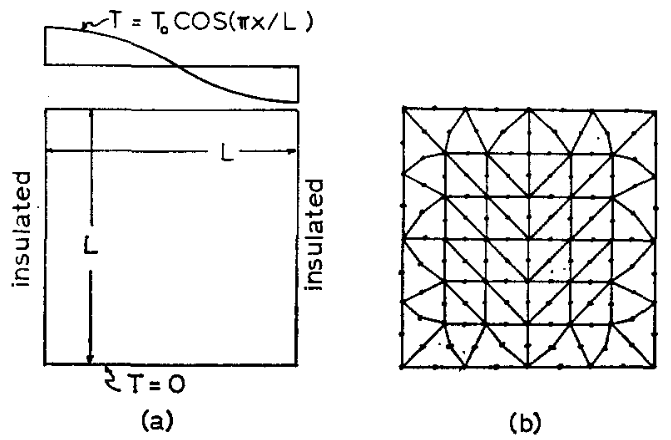
\includegraphics[width=6cm]{python_codes/fieldstone_38/images/sath76_a}
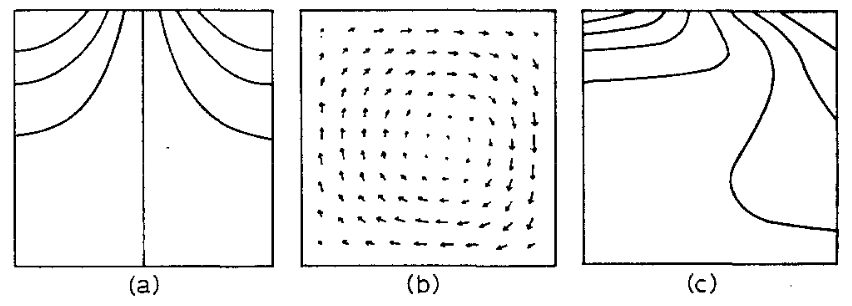
\includegraphics[width=8cm]{python_codes/fieldstone_38/images/sath76_b}\\
{\captionfont Left: (a) Boundary conditions; (b) Mesh layout - the authors
use $P_2\times P_1$ elements;\\
Right: Isotherms and velocity field: (a) Steady-state conduction;
velocity field; (c) Steady-state isotherms R = 4580.}
\end{center}

The code is based on \stone~03, and because velocities are very small for low Rayleigh numbers
reduced densities are used, i.e. the buoyancy force in the Stokes equation is given by $-\alpha(T-T_0)\vec{g}$.
Steady state is reached when the velocity and temperature fields do not change by more than $tol=10^{-6}$.

Note that what is called Nu in the code is in fact $Q=\int_0^{L_x} q_y dx$.

I have also run the very same experiments with \aspect{} at mesh uniform level 5 (and found that 
level 6 did not change anything to the results). The prm file is hereby joined to this repository.

As explained in McKenzie \etal (1974), for $\Ranb <<1$ advection of heat is negligible and $T$ is therefore harmonic:
\[
T(x,y) = \Delta T \cos (\pi x/L) \frac{\sinh \pi z/L}{\sinh \pi L_y/L_x}
\]
When $T_0=0.01$, only heat diffusion is present and we recover the analytical solution presented in McKenzie \etal:

\begin{center}
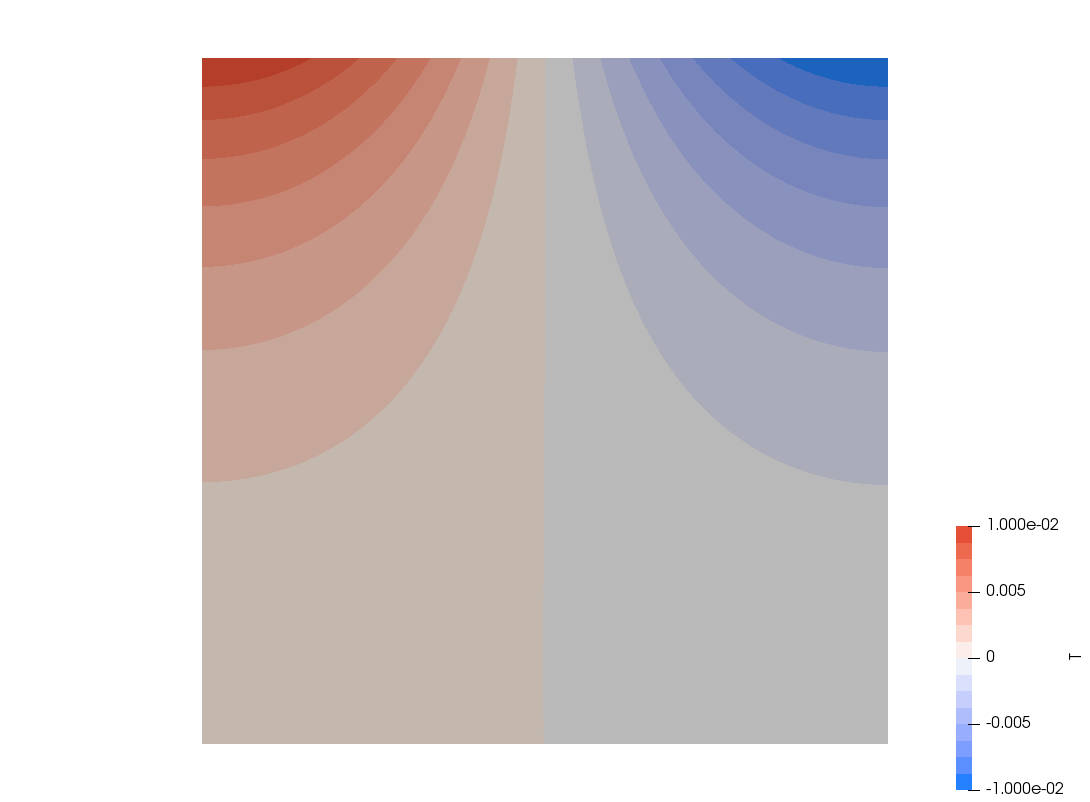
\includegraphics[width=6cm]{python_codes/fieldstone_38/results/T0_0p001_32x32/T}
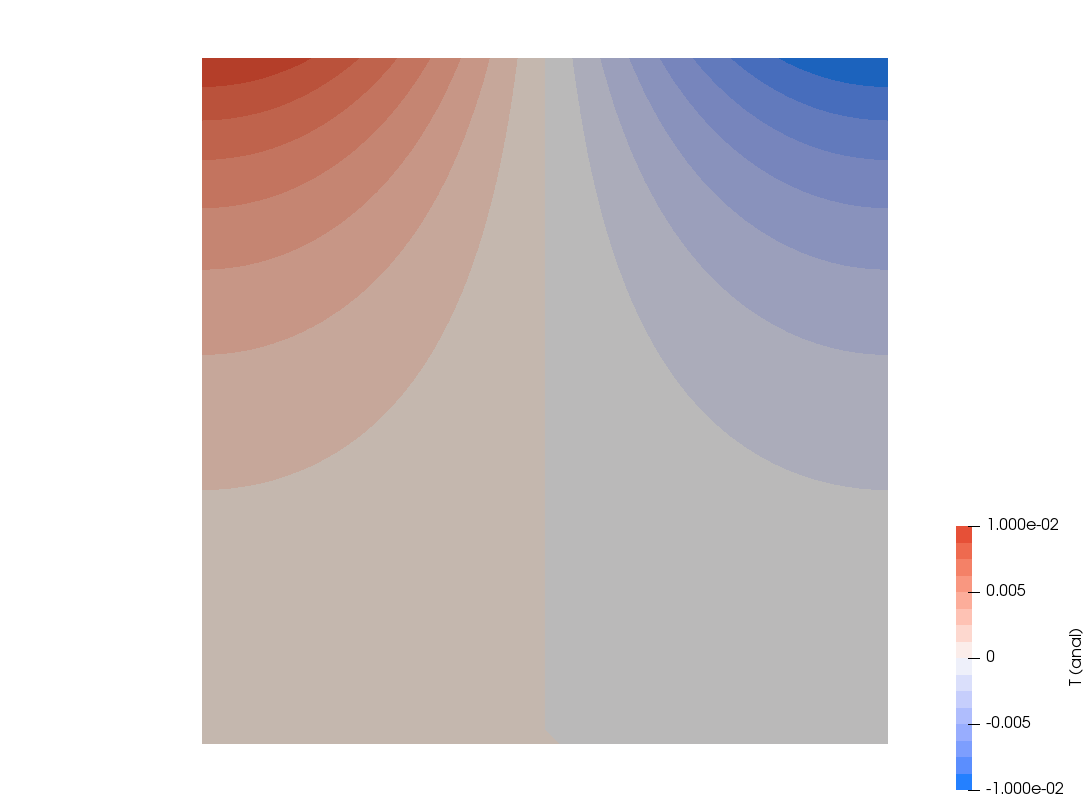
\includegraphics[width=6cm]{python_codes/fieldstone_38/results/T0_0p001_32x32/T_anal}\\
{\captionfont Left: computed temperature, 48x48 resolution; Right: analytical solution.}
\end{center}

\newpage
\subsubsection*{Steady-state study}


\begin{center}
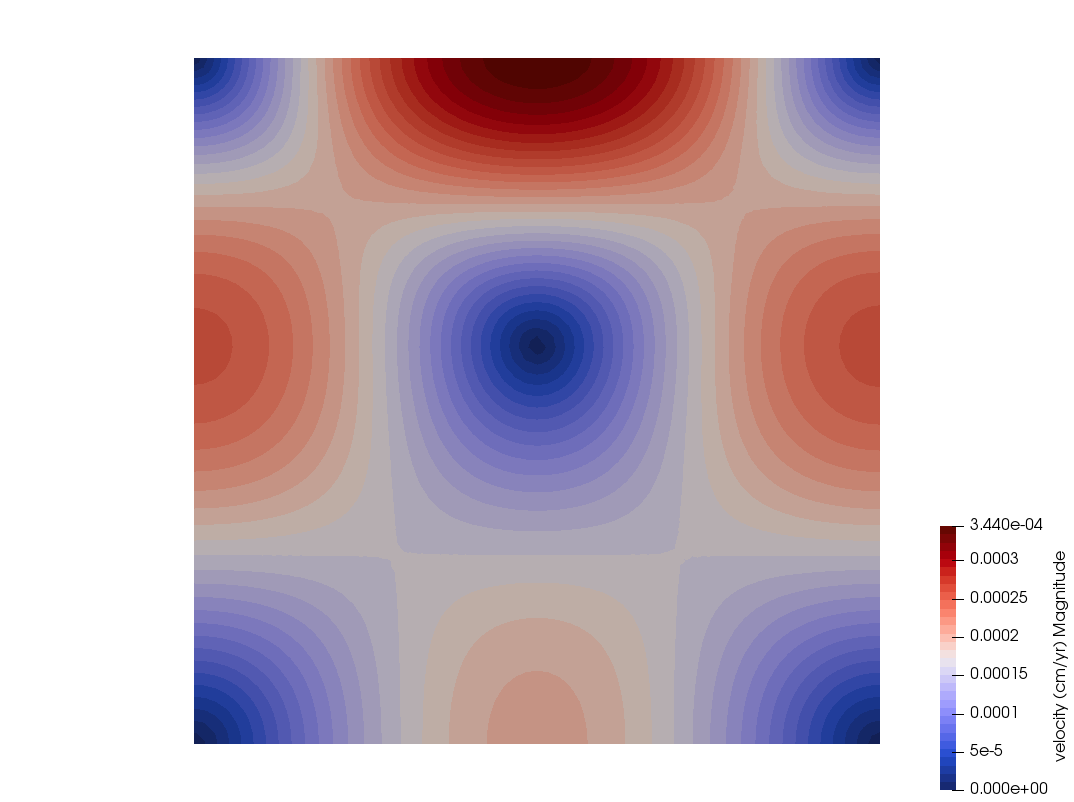
\includegraphics[height=4cm]{python_codes/fieldstone_38/results/T0_0p01_64x64/vel}
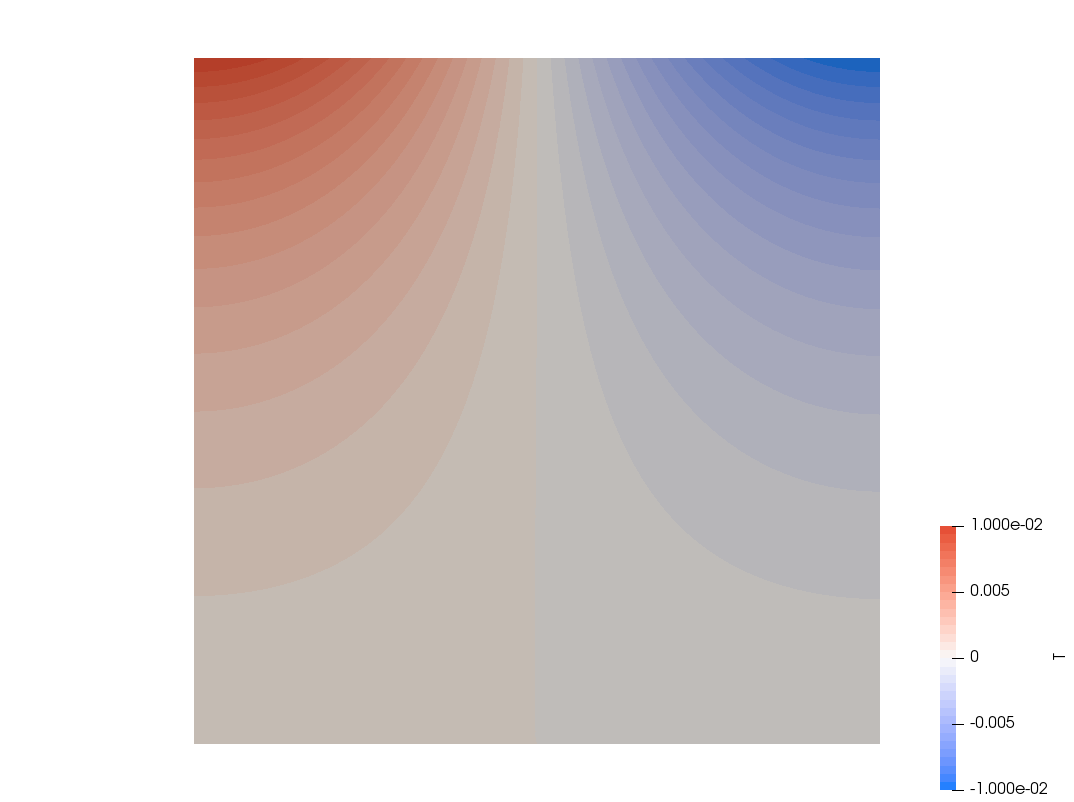
\includegraphics[height=4cm]{python_codes/fieldstone_38/results/T0_0p01_64x64/T}
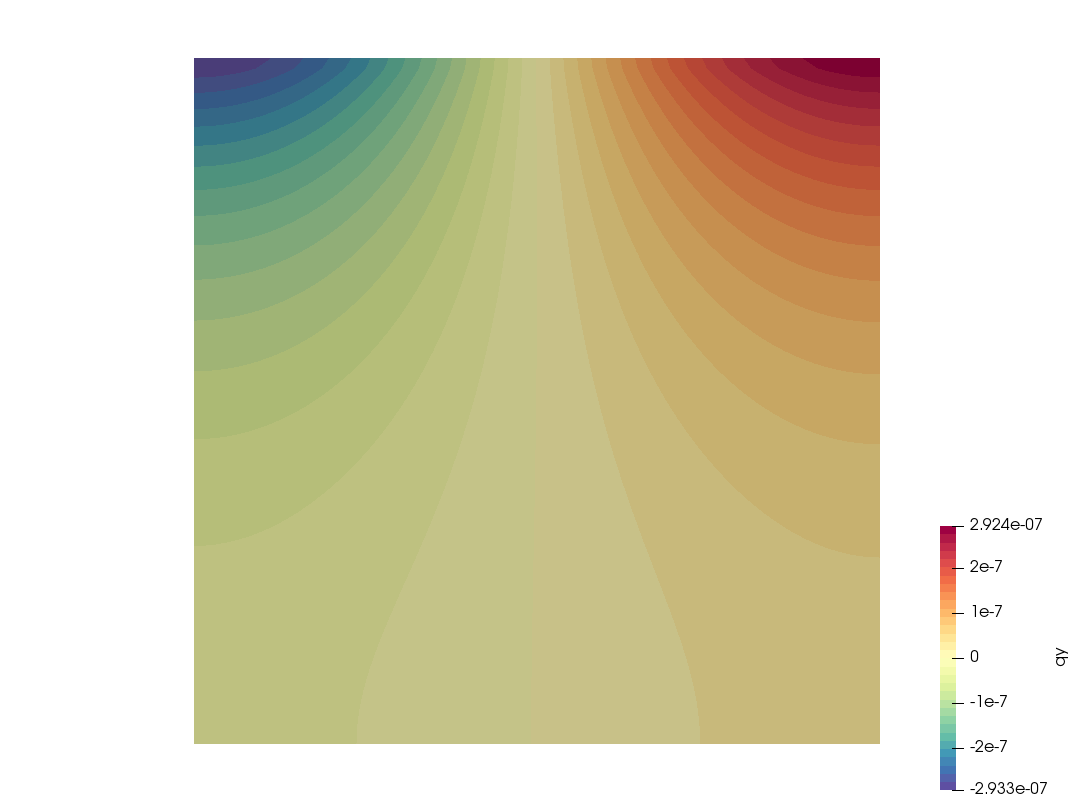
\includegraphics[height=4cm]{python_codes/fieldstone_38/results/T0_0p01_64x64/qy}\\
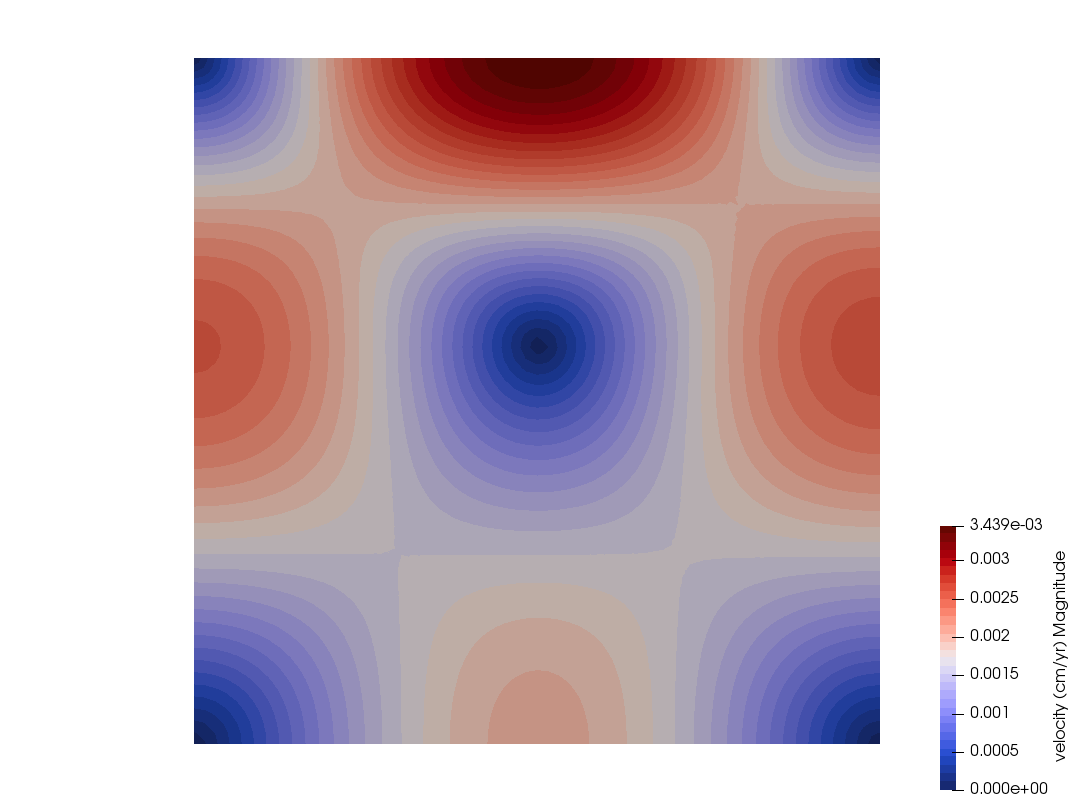
\includegraphics[height=4cm]{python_codes/fieldstone_38/results/T0_0p1_64x64/vel}
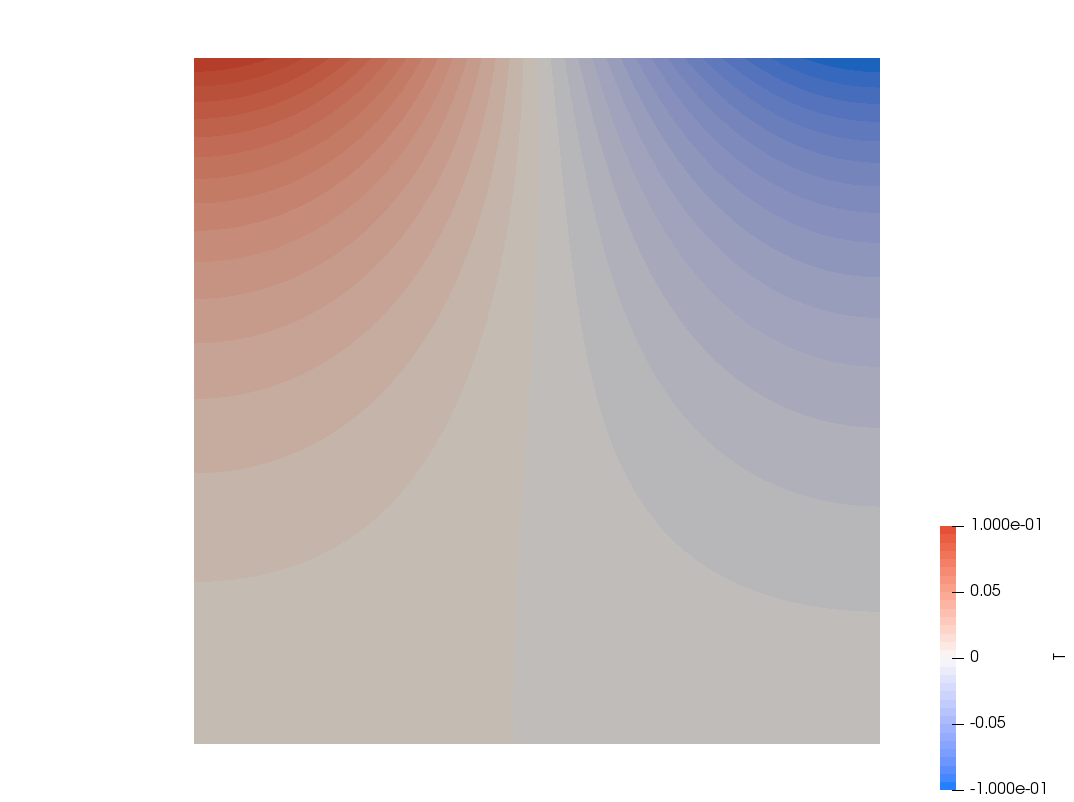
\includegraphics[height=4cm]{python_codes/fieldstone_38/results/T0_0p1_64x64/T}
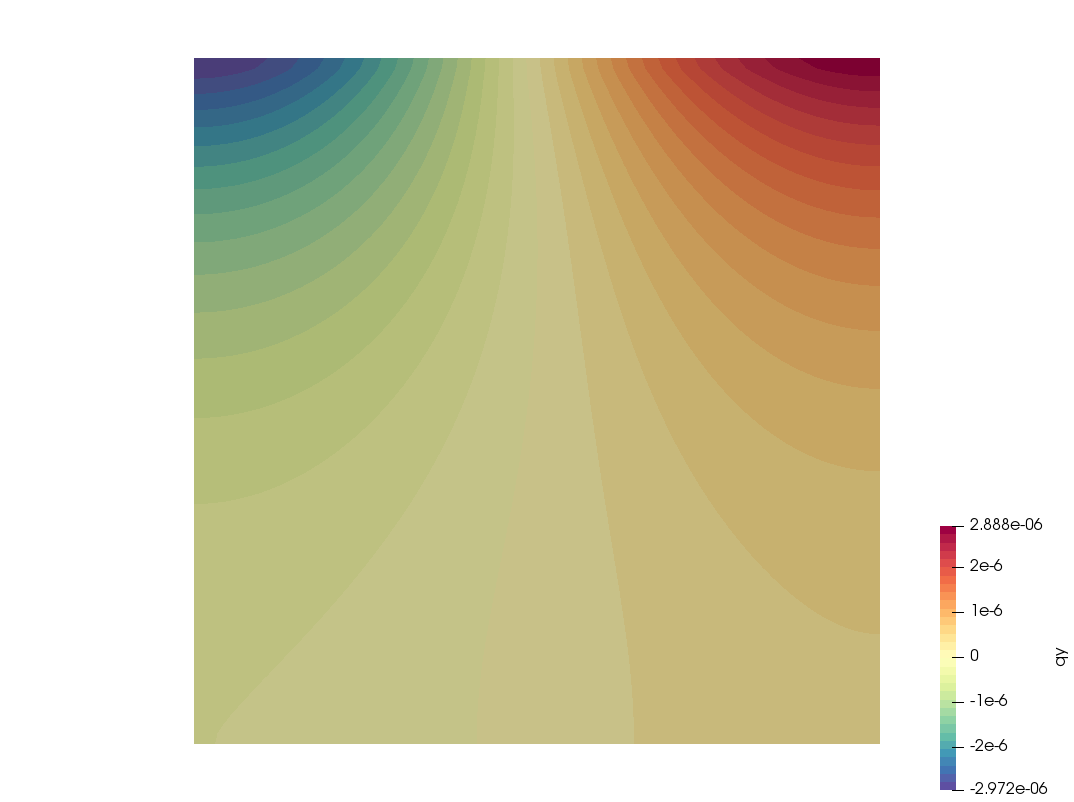
\includegraphics[height=4cm]{python_codes/fieldstone_38/results/T0_0p1_64x64/qy}\\
missing T0=1 \\
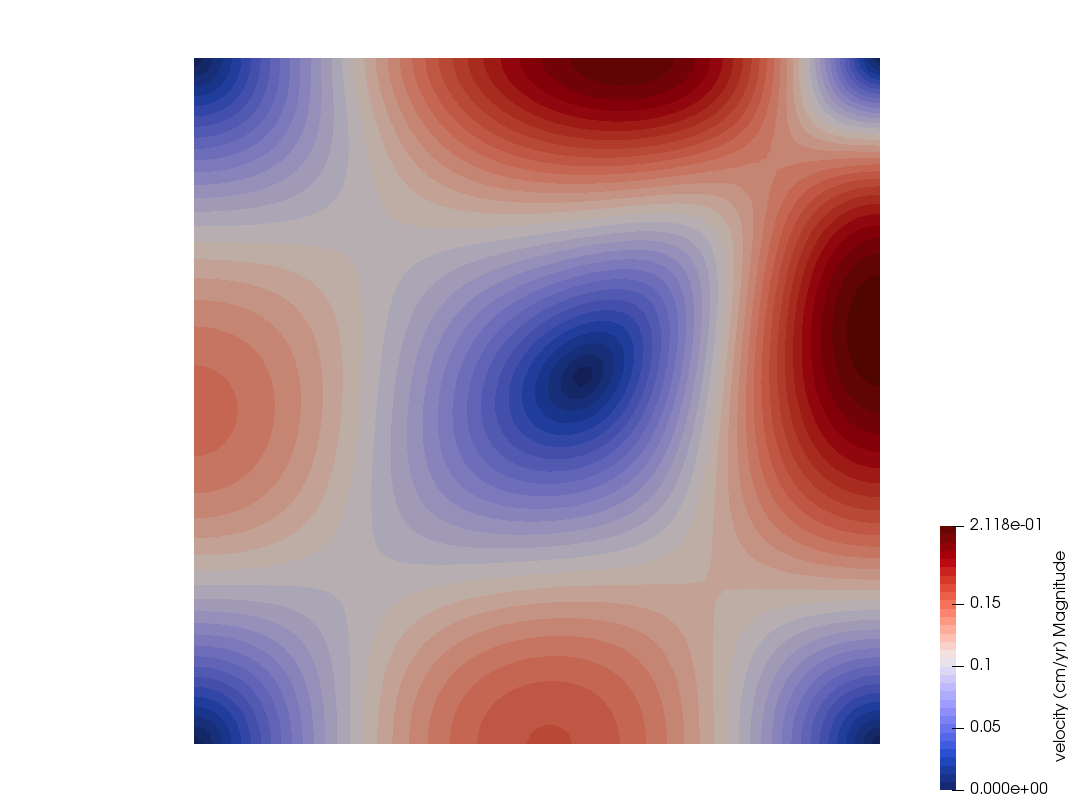
\includegraphics[height=4cm]{python_codes/fieldstone_38/results/T0_10_64x64/vel}
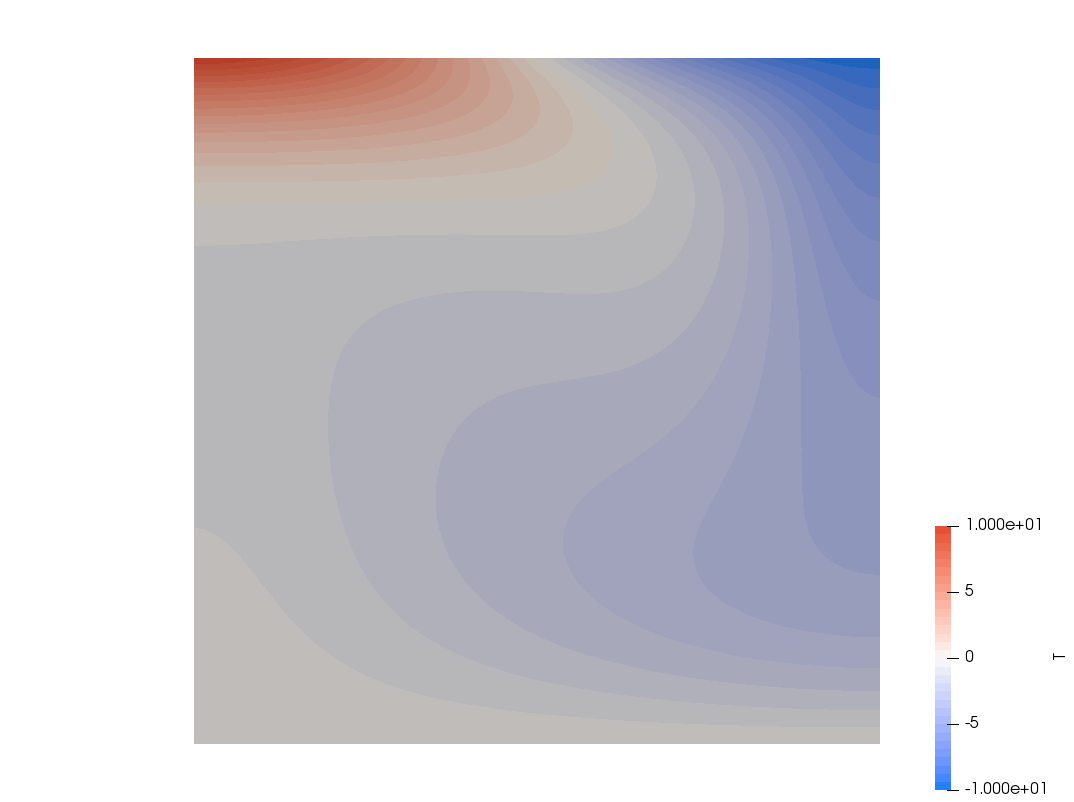
\includegraphics[height=4cm]{python_codes/fieldstone_38/results/T0_10_64x64/T}
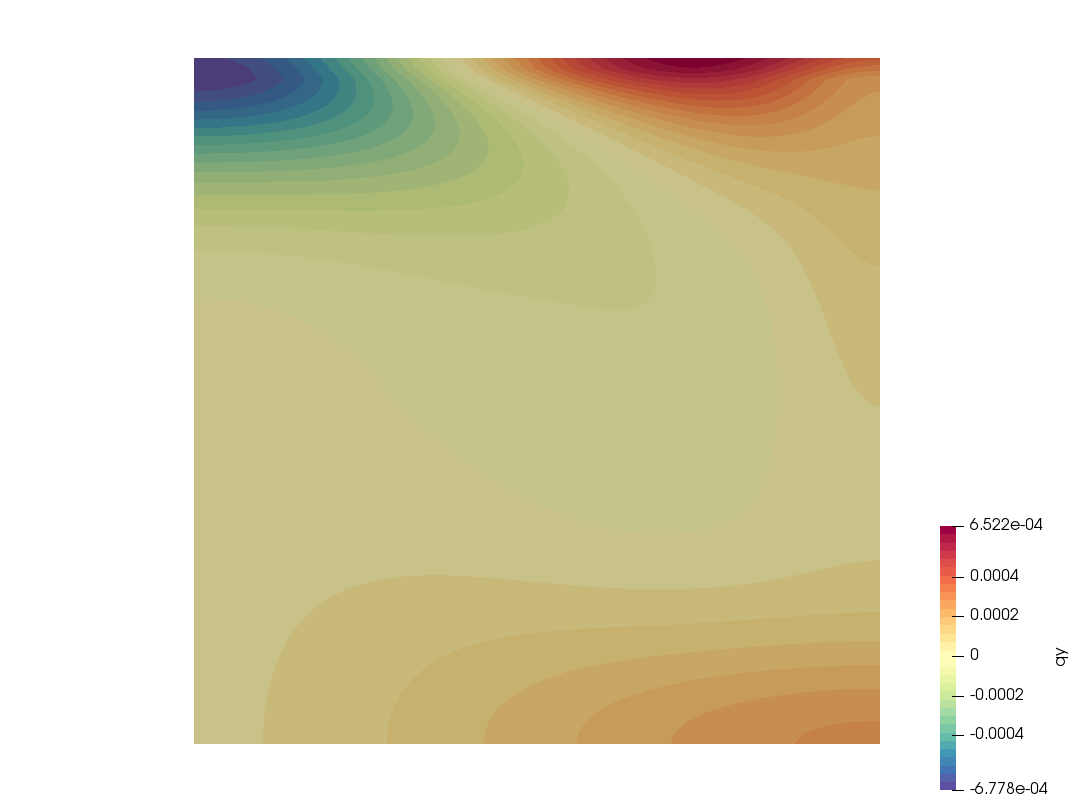
\includegraphics[height=4cm]{python_codes/fieldstone_38/results/T0_10_64x64/qy}\\
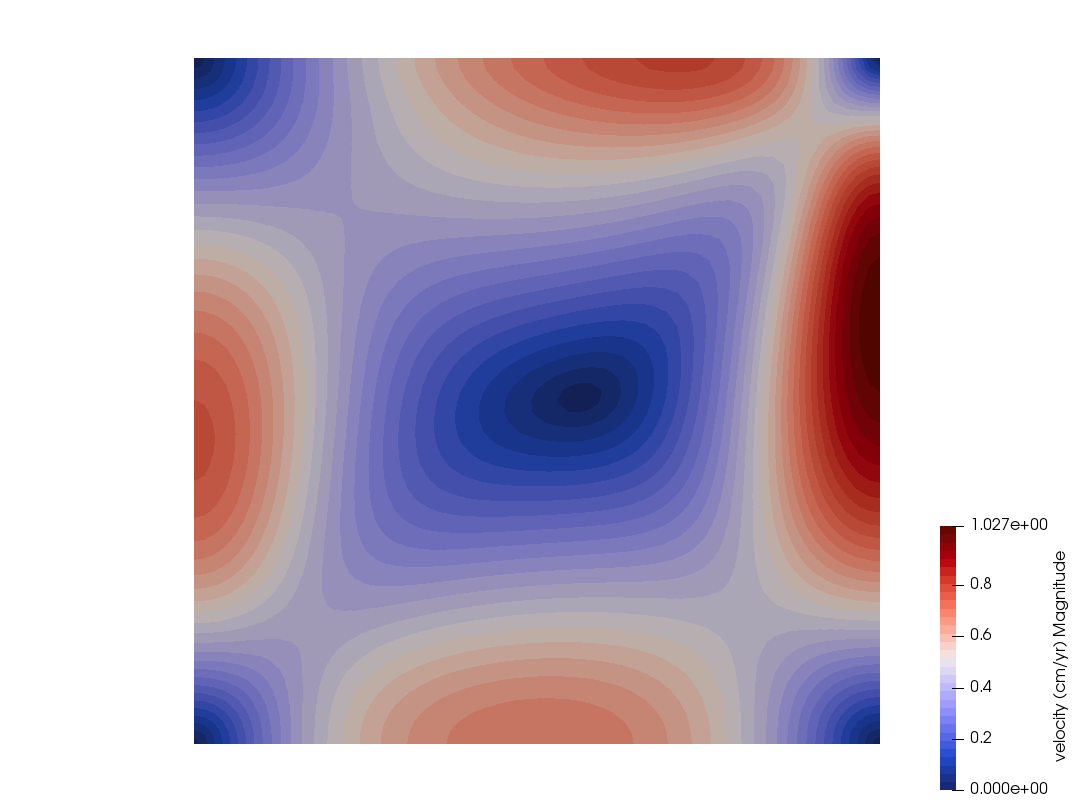
\includegraphics[height=4cm]{python_codes/fieldstone_38/results/T0_100_64x64/vel}
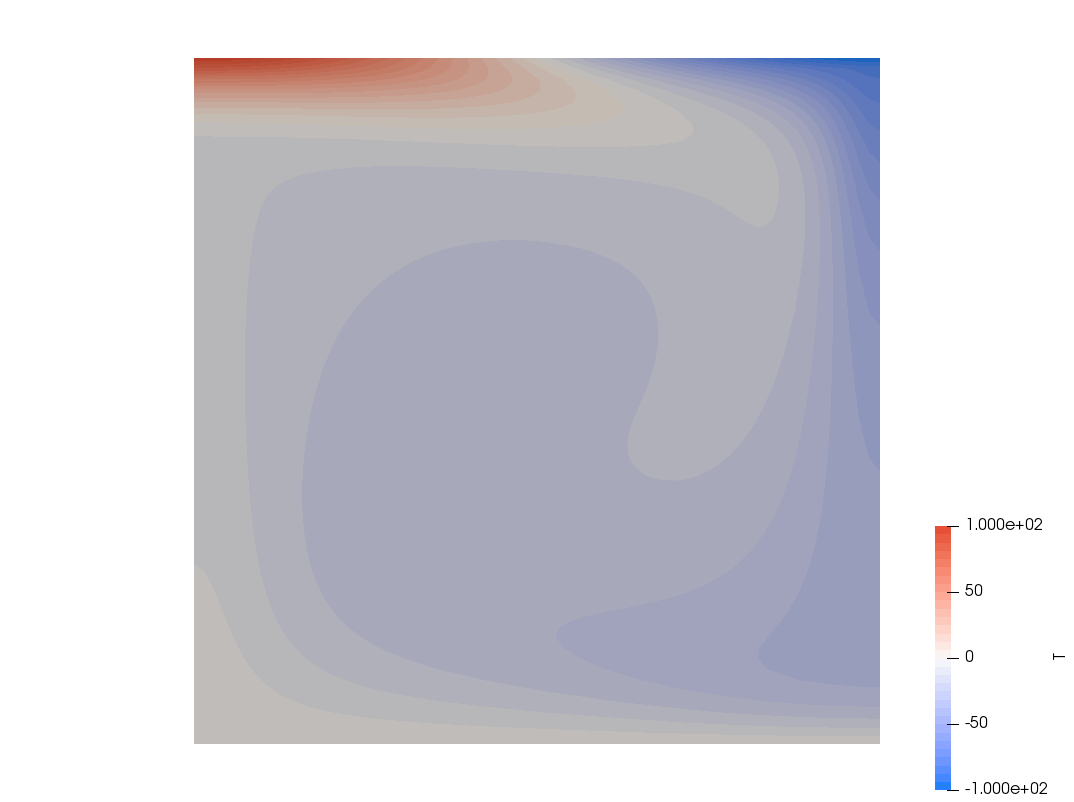
\includegraphics[height=4cm]{python_codes/fieldstone_38/results/T0_100_64x64/T}
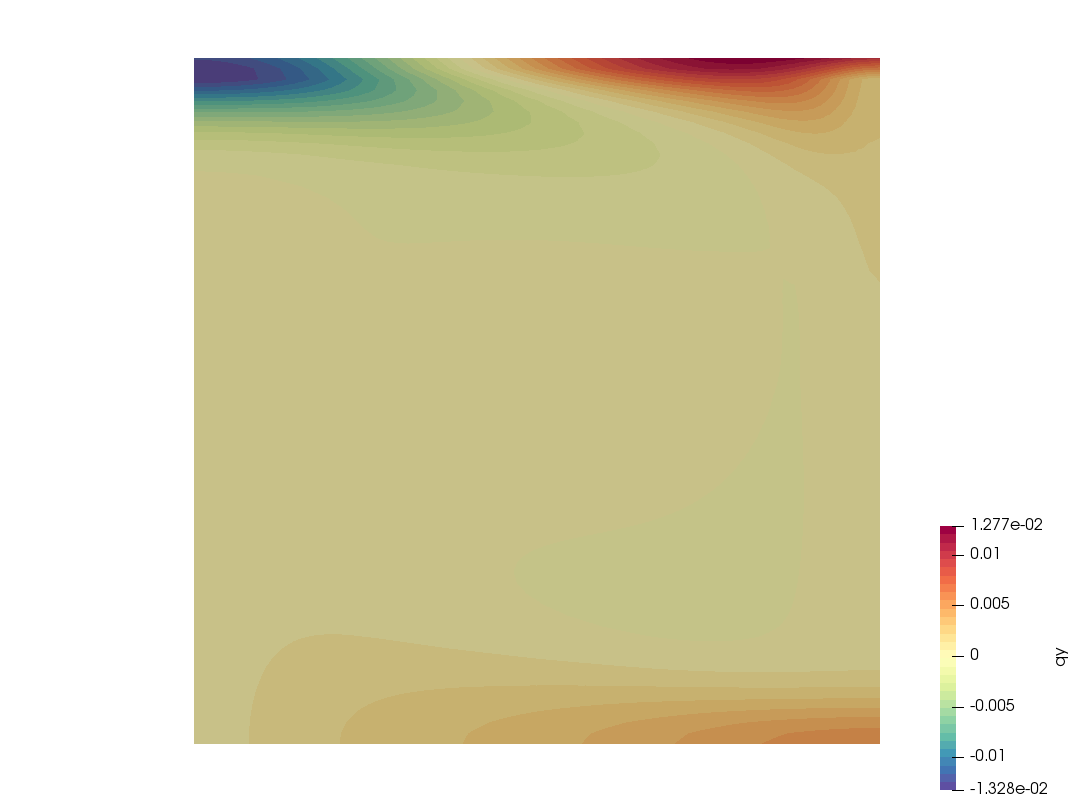
\includegraphics[height=4cm]{python_codes/fieldstone_38/results/T0_100_64x64/qy}\\
{\captionfont Obtained with \stone~38 on 64x64 mesh. 
Top to bottom: $T_0=0.01,0.1,1,10,100$}
\end{center}

\newpage
\begin{center}
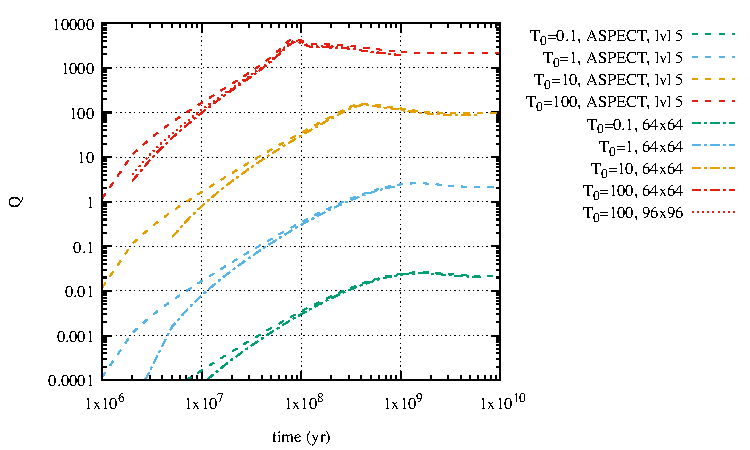
\includegraphics[width=13cm]{python_codes/fieldstone_38/results/Q.pdf}\\
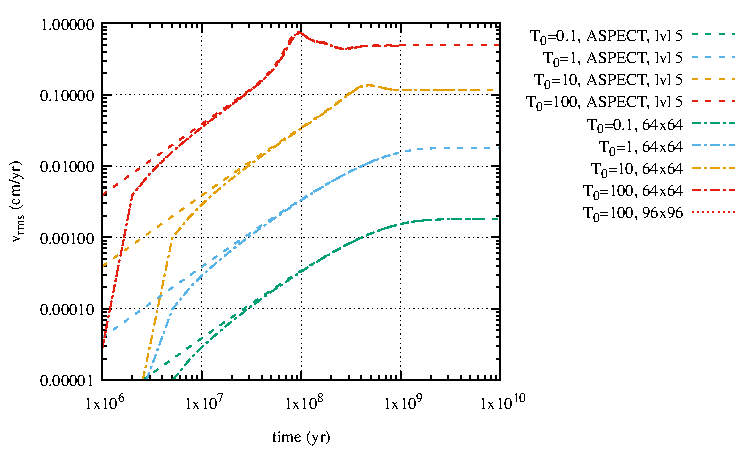
\includegraphics[width=13cm]{python_codes/fieldstone_38/results/vrms.pdf}\\
{\captionfont Heat flux on top boundary (top) and root mean square velocity (bottom)
as measured with \stone~38 and \aspect on 64x64 mesh.}
\end{center}

TODO: boundary conditions should be done on elemental matrices.




